%%%%%%%%%%%%%%%%%%%%%%%%%%%%%%%%%%%%%%%%%%%%%%%%%%%%%%%%%%%%%%%%%%%%%%%%%%%
%% This file is part of the book
%%
%% Algorithmic Graph Theory
%% http://code.google.com/p/graph-theory-algorithms-book/
%%
%% Copyright (C) 2009, 2010 Minh Van Nguyen <nguyenminh2@gmail.com>
%%
%% See the file COPYING for copying conditions.
%%%%%%%%%%%%%%%%%%%%%%%%%%%%%%%%%%%%%%%%%%%%%%%%%%%%%%%%%%%%%%%%%%%%%%%%%%%

\subfigure[Original digraph.]{
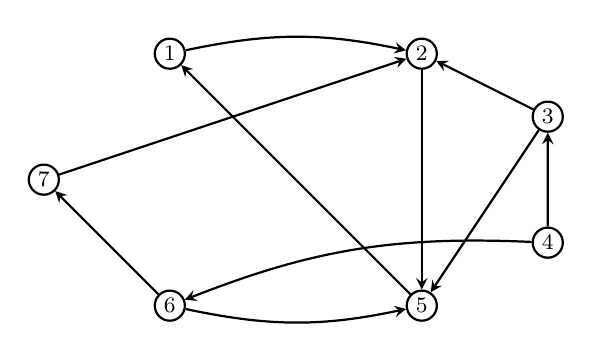
\begin{tikzpicture}
[arrowDecorate/.style={->,>=stealth,thick},%
  nodeDecorate/.style={shape=circle,inner sep=1.5pt,draw,thick},%
  scale=0.8]
%% nodes or vertices
\foreach \nodename/\x/\y in {2/4/4, 1/0/4, 3/6/3, 4/6/1, 5/4/0, 7/-2/2, 6/0/0}
{
  \node (\nodename) at (\x,\y) [nodeDecorate] {\footnotesize$\nodename$};
}
%% edges or lines
\path
\foreach \startnode/\endnode in {2/5, 3/2, 3/5, 4/3, 5/1, 6/7, 7/2}
{
  (\startnode) edge[arrowDecorate] node {} (\endnode)
}
\foreach \startnode/\endnode/\benddirection/\angle in {
  1/2/bend left/12, 4/6/bend right/12, 6/5/bend right/12}
{
  (\startnode) edge[arrowDecorate,\benddirection=\angle] node {} (\endnode)
};
\end{tikzpicture}
}
%%
%%
\qquad
\subfigure[First iteration of while loop.]{
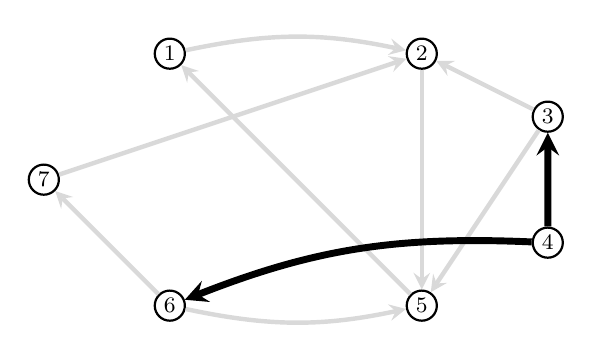
\begin{tikzpicture}
[darkArrow/.style={->,>=stealth,line width=2.5pt},%
  lightArrow/.style={->,>=stealth,ultra thick,color=gray!30},%
  nodeDecorate/.style={shape=circle,inner sep=1.5pt,draw,thick},%
  scale=0.8]
%% nodes or vertices
\foreach \nodename/\x/\y in {2/4/4, 1/0/4, 3/6/3, 4/6/1, 5/4/0, 7/-2/2, 6/0/0}
{
  \node (\nodename) at (\x,\y) [nodeDecorate] {\footnotesize$\nodename$};
}
%% light edges or lines
\path
\foreach \startnode/\endnode in {2/5, 3/2, 3/5, 5/1, 6/7, 7/2}
{
  (\startnode) edge[lightArrow] node {} (\endnode)
}
\foreach \startnode/\endnode/\benddirection/\angle in {
  1/2/bend left/12, 6/5/bend right/12}
{
  (\startnode) edge[lightArrow,\benddirection=\angle] node {} (\endnode)
}
%% dark edges or lines
\foreach \startnode/\endnode in {4/3}
{
  (\startnode) edge[darkArrow] node {} (\endnode)
}
\foreach \startnode/\endnode/\benddirection/\angle in {4/6/bend right/12}
{
  (\startnode) edge[darkArrow,\benddirection=\angle] node {} (\endnode)
};
\end{tikzpicture}
}
%%
%%
\subfigure[Second iteration of while loop.]{
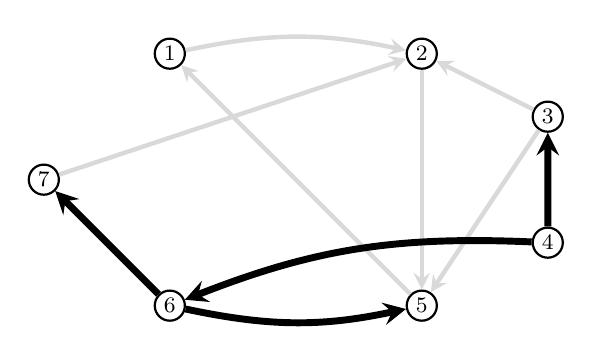
\begin{tikzpicture}
[darkArrow/.style={->,>=stealth,line width=2.5pt},%
  lightArrow/.style={->,>=stealth,ultra thick,color=gray!30},%
  nodeDecorate/.style={shape=circle,inner sep=1.5pt,draw,thick},%
  scale=0.8]
%% nodes or vertices
\foreach \nodename/\x/\y in {2/4/4, 1/0/4, 3/6/3, 4/6/1, 5/4/0, 7/-2/2, 6/0/0}
{
  \node (\nodename) at (\x,\y) [nodeDecorate] {\footnotesize$\nodename$};
}
%% light edges or lines
\path
\foreach \startnode/\endnode in {2/5, 3/2, 3/5, 5/1, 7/2}
{
  (\startnode) edge[lightArrow] node {} (\endnode)
}
\foreach \startnode/\endnode/\benddirection/\angle in {1/2/bend left/12}
{
  (\startnode) edge[lightArrow,\benddirection=\angle] node {} (\endnode)
}
%% dark edges or lines
\foreach \startnode/\endnode in {4/3, 6/7}
{
  (\startnode) edge[darkArrow] node {} (\endnode)
}
\foreach \startnode/\endnode/\benddirection/\angle in {
  4/6/bend right/12, 6/5/bend right/12}
{
  (\startnode) edge[darkArrow,\benddirection=\angle] node {} (\endnode)
};
\end{tikzpicture}
}
%%
%%
\qquad
\subfigure[Third iteration of while loop.]{
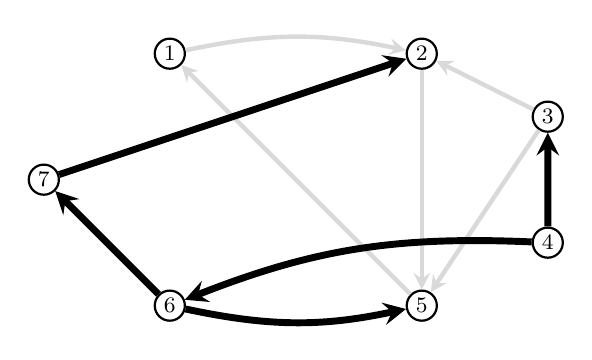
\begin{tikzpicture}
[darkArrow/.style={->,>=stealth,line width=2.5pt},%
  lightArrow/.style={->,>=stealth,ultra thick,color=gray!30},%
  nodeDecorate/.style={shape=circle,inner sep=1.5pt,draw,thick},%
  scale=0.8]
%% nodes or vertices
\foreach \nodename/\x/\y in {2/4/4, 1/0/4, 3/6/3, 4/6/1, 5/4/0, 7/-2/2, 6/0/0}
{
  \node (\nodename) at (\x,\y) [nodeDecorate] {\footnotesize$\nodename$};
}
%% light edges or lines
\path
\foreach \startnode/\endnode in {2/5, 3/2, 3/5, 5/1}
{
  (\startnode) edge[lightArrow] node {} (\endnode)
}
\foreach \startnode/\endnode/\benddirection/\angle in {1/2/bend left/12}
{
  (\startnode) edge[lightArrow,\benddirection=\angle] node {} (\endnode)
}
%% dark edges or lines
\foreach \startnode/\endnode in {4/3, 6/7, 7/2}
{
  (\startnode) edge[darkArrow] node {} (\endnode)
}
\foreach \startnode/\endnode/\benddirection/\angle in {
  4/6/bend right/12, 6/5/bend right/12}
{
  (\startnode) edge[darkArrow,\benddirection=\angle] node {} (\endnode)
};
\end{tikzpicture}
}
%%
%%
\subfigure[Fourth iteration of while loop.]{
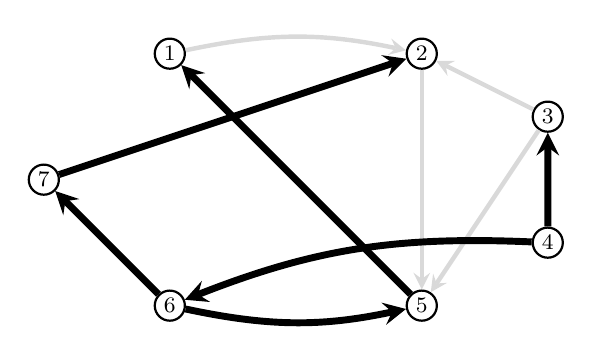
\begin{tikzpicture}
[darkArrow/.style={->,>=stealth,line width=2.5pt},%
  lightArrow/.style={->,>=stealth,ultra thick,color=gray!30},%
  nodeDecorate/.style={shape=circle,inner sep=1.5pt,draw,thick},%
  scale=0.8]
%% nodes or vertices
\foreach \nodename/\x/\y in {2/4/4, 1/0/4, 3/6/3, 4/6/1, 5/4/0, 7/-2/2, 6/0/0}
{
  \node (\nodename) at (\x,\y) [nodeDecorate] {\footnotesize$\nodename$};
}
%% light edges or lines
\path
\foreach \startnode/\endnode in {2/5, 3/2, 3/5}
{
  (\startnode) edge[lightArrow] node {} (\endnode)
}
\foreach \startnode/\endnode/\benddirection/\angle in {1/2/bend left/12}
{
  (\startnode) edge[lightArrow,\benddirection=\angle] node {} (\endnode)
}
%% dark edges or lines
\foreach \startnode/\endnode in {4/3, 5/1, 6/7, 7/2}
{
  (\startnode) edge[darkArrow] node {} (\endnode)
}
\foreach \startnode/\endnode/\benddirection/\angle in {
  4/6/bend right/12, 6/5/bend right/12}
{
  (\startnode) edge[darkArrow,\benddirection=\angle] node {} (\endnode)
};
\end{tikzpicture}
}
%%
%%
\qquad
\subfigure[Final DFS tree.]{
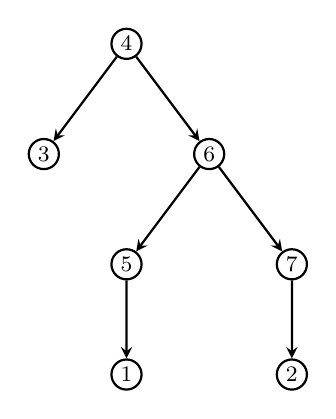
\begin{tikzpicture}
[arrowDecorate/.style={->,>=stealth,thick},%
  nodeDecorate/.style={shape=circle,inner sep=1.5pt,draw,thick},%
  scale=1.4]
%% nodes or vertices
\foreach \nodename/\x/\y in {
  4/1.25/3, 3/0.5/2, 6/2/2, 5/1.25/1, 7/2.75/1, 1/1.25/0, 2/2.75/0}
{
  \node (\nodename) at (\x,\y) [nodeDecorate] {\footnotesize$\nodename$};
}
%% edges or lines
\path
\foreach \startnode/\endnode in {4/3, 4/6, 6/5, 6/7, 5/1, 7/2}
{
  (\startnode) edge[arrowDecorate] node {} (\endnode)
};
\end{tikzpicture}
}
